The rapid adoption of Large Language Models (LLMs) has fundamentally transformed software development, shifting it from a primarily generative activity to one centered on evaluating and curating AI-generated solutions. This transition represents not just a technological shift, but a deeper cognitive change in how developers approach problem-solving and decision-making. As developers increasingly rely on AI tools—used by over 90\% of practitioners—they must interpret, validate, and integrate machine-generated outputs into their workflows. This evolving paradigm introduces new cognitive demands, raising important questions about how human reasoning interacts with AI assistance and how decision quality is affected in such collaborative environments.

At the core of this transformation lies the role of cognitive biases—systematic deviations from rational thinking that influence human judgment. While such biases have long been present in traditional software engineering (e.g., confirmation bias or anchoring), LLM-assisted development creates a new landscape where these biases may be amplified or take entirely new forms. Developers must now navigate challenges such as over-reliance on AI suggestions, ineffective prompt formulation, and misinterpretation of generated outputs. Despite the widespread integration of LLMs, there has been little systematic understanding of how these biases manifest in human-AI collaboration. This paper addresses this gap by investigating cognitive biases in LLM-assisted programming and highlighting their implications for software quality, developer productivity, and decision-making in modern development workflows.

\section{Motivation}
The motivation for this paper arises from the fundamental transformation of software development driven by the rapid adoption of LLM-based coding tools. With over \% of developers now using AI assistants \cite{github2023copilot}, programming has shifted from a purely generative activity to one centered on \textbf{evaluation, validation, and integration of AI-generated code}. This shift represents a \textbf{cognitive paradigm change}, where developers must continuously interpret and judge machine outputs rather than construct solutions from scratch. While such assistance improves productivity, it also introduces new cognitive demands that place greater reliance on human judgment under uncertainty. Since human reasoning is inherently subject to biases—systematic deviations from rational thinking that influence decision-making \cite{tversky1974judgment, kahneman2011thinking}—this evolving workflow raises concerns about the quality and reliability of decisions made in AI-assisted environments.

In traditional software engineering, cognitive biases have been extensively studied and shown to affect various stages of development. For example, developers often exhibit \textbf{confirmation bias by favoring solutions aligned with prior beliefs}, \textbf{anchoring bias by relying heavily on initial ideas}, and \textbf{availability bias by overemphasizing recent experiences} \cite{mohanani2018cognitive, chattopadhyay2020cognitive}. These biases can lead to suboptimal design decisions, overlooked defects, and inefficient problem-solving. However, the introduction of LLMs fundamentally alters the decision-making landscape. Developers must now \textbf{formulate prompts, evaluate multiple AI-generated alternatives, and reconcile conflicting outputs}, creating new opportunities for bias to emerge or intensify. The paper is motivated by the hypothesis that \textbf{LLM-assisted development not only preserves existing biases but amplifies them and introduces entirely new bias patterns specific to human-AI collaboration} .

A key concern driving this work is the potential impact of biased decision-making on software quality and long-term system health. In LLM-assisted workflows, \textbf{biased judgments can propagate through entire codebases}, leading to subtle bugs, security vulnerabilities, and accumulating technical debt that may not be immediately visible . Moreover, recent research suggests that reliance on AI systems can reduce critical thinking and increase susceptibility to cognitive biases \cite{lee2025impact}. This phenomenon of cognitive offloading implies that developers may \textbf{over-trust AI-generated solutions or accept outputs without sufficient scrutiny}, further compounding risks. As LLMs become deeply embedded in development pipelines, understanding these cognitive implications becomes essential for ensuring \textbf{robust, secure, and maintainable software systems}.

From a related work perspective, prior research has explored cognitive biases extensively in both software engineering and broader human-AI interaction contexts. Systematic studies have cataloged numerous biases affecting developers, providing taxonomies and evidence of their impact on software processes \cite{mohanani2018cognitive}. Similarly, work on human-AI collaboration has examined how users interact with intelligent systems and how biases influence trust, reliance, and decision-making \cite{lee2025impact}. However, \textbf{no prior work has systematically investigated cognitive biases in real-world LLM-assisted programming environments} . Existing bias taxonomies were developed for pre-LLM settings and may not adequately capture challenges such as prompt engineering, iterative AI interaction, and evaluation of generated code. This creates a significant research gap, leaving practitioners without \textbf{evidence-based guidelines to mitigate bias in AI-assisted development workflows}.

Therefore, the paper is motivated by the need to bridge this gap through a comprehensive empirical investigation of cognitive biases in LLM-assisted programming. By identifying how biases manifest, evolve, and impact developer decisions in these new environments, the work aims to provide \textbf{actionable insights for improving developer decision-making, enhancing tool design, and mitigating risks associated with AI-assisted coding}. Ultimately, this research is driven by the broader goal of ensuring that the integration of LLMs into software engineering enhances productivity without compromising \textbf{decision quality, software reliability, and developer cognition}.

\section{Methodology}
\begin{figure}
    \centering
    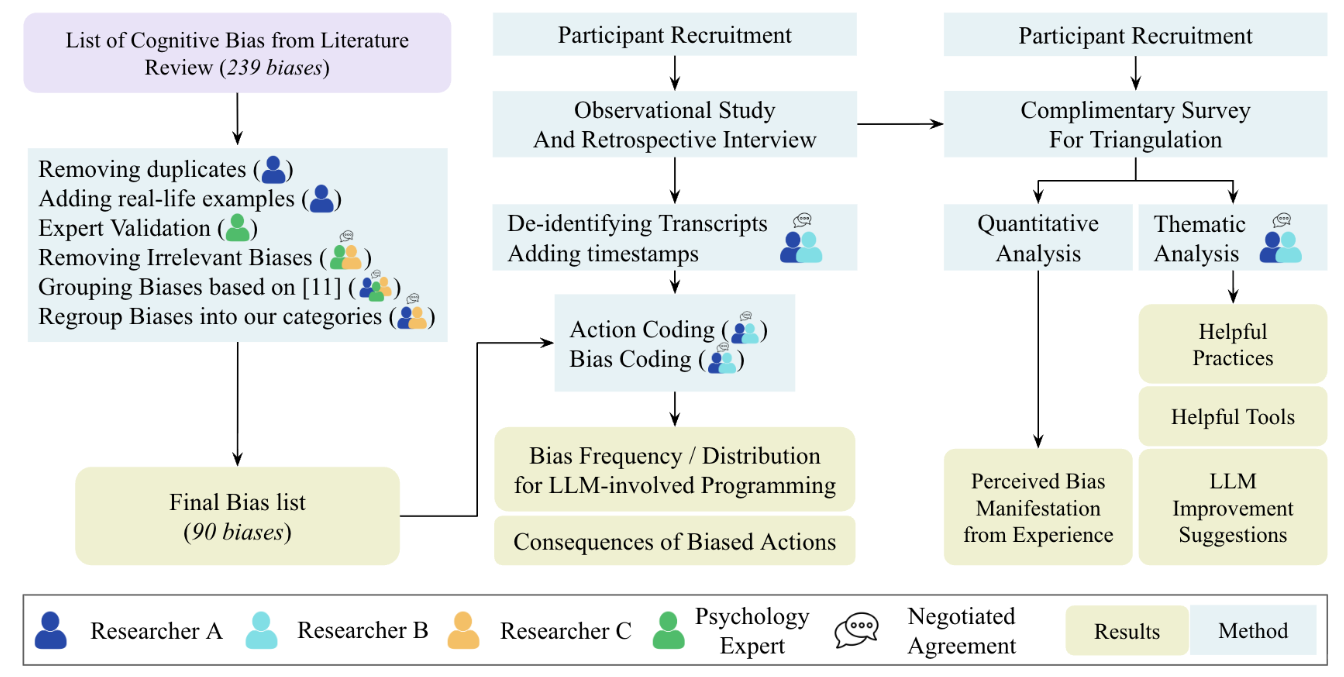
\includegraphics[width=0.9\textwidth]{methodology_overview.png}
    \caption{Methodology Overview}
    \label{fig:bias_taxonomy}
\end{figure}
\subsection{Study Design and Research Approach}
The paper adopts a mixed-method empirical research design to investigate cognitive biases in LLM-assisted software development. The authors combine observational studies with retrospective interviews and surveys to ensure a comprehensive understanding of developer behavior. Specifically, the study is designed to \textbf{capture real-world developer interactions with LLM tools}, rather than relying on controlled or synthetic tasks. This approach enables the authors to analyze how cognitive biases emerge naturally during programming activities and how they influence decision-making in practice. To ground their analysis, the study initially leverages an existing bias taxonomy from prior software engineering research \cite{chattopadhyay2020cognitive}, ensuring continuity with established literature while enabling comparison with pre-LLM contexts.

\subsection{Participants and Data Collection}
The study involves a total of \textbf{14 participants, including both students and professional developers}, ensuring diversity in experience levels and development practices. Data collection is centered around detailed observational sessions in which participants perform programming tasks while interacting with LLM tools. Across these sessions, the authors record \textbf{2,013 development actions}, of which \textbf{808 involve direct LLM interactions} . This fine-grained logging allows the researchers to analyze developer behavior at the level of individual actions, capturing how decisions evolve over time.

To complement observational data, the study incorporates \textbf{retrospective interviews}, enabling participants to reflect on their decision-making processes and provide insights into their reasoning. Additionally, the authors conduct \textbf{confirmatory surveys with 22 developers} to triangulate findings and validate observed patterns across a broader population . This multi-source data collection strategy strengthens the validity of the study by combining behavioral evidence with self-reported insights.

\subsection{Bias Identification and Analytical Framework}
The methodology begins with the application of an existing cognitive bias framework proposed by Chattopadhyay et al. \cite{chattopadhyay2020cognitive}. Using this framework, the authors systematically analyze developer actions to identify instances of bias. Each recorded action is examined to determine whether it reflects a deviation from rational decision-making, allowing the researchers to \textbf{quantify the prevalence of cognitive biases in LLM-assisted programming}.

However, the study goes beyond simple classification by investigating the relationship between biased actions and their outcomes. In particular, the authors analyze \textbf{reversal actions}—instances where developers undo or revise prior decisions—to assess whether biased decisions are more likely to be corrected. Statistical analysis, including chi-square tests with Bonferroni corrections, is used to evaluate the significance of observed patterns. The findings reveal that \textbf{LLM-related actions are more likely to be biased (53.7\%) and more likely to be reversed (29.4\%)}, highlighting the complex interplay between AI assistance and human judgment.

\subsubsection{Development of Bias Taxonomy}
A key methodological contribution of the paper is the development of a new taxonomy tailored to LLM-assisted programming. Recognizing that existing bias categories may be insufficient, the authors conduct a systematic analysis of \textbf{90 cognitive biases relevant to developer–LLM interactions} and organize them into \textbf{15 distinct categories} . This categorization is achieved through a negotiated agreement process with cognitive science experts, ensuring theoretical rigor and domain validity.

The resulting taxonomy captures both traditional biases (e.g., confirmation and anchoring) and novel biases emerging from human-AI interaction, such as \textbf{suggester preference and humanization of LLMs}. This step is crucial as it allows the study to move beyond existing frameworks and \textbf{identify new cognitive patterns unique to AI-assisted development}. The taxonomy serves as the foundation for subsequent analysis, enabling a more accurate characterization of developer behavior in LLM-driven workflows.

\subsubsection{Triangulation and Validation}
To ensure robustness, the study employs multiple forms of triangulation. First, observational data is cross-validated with retrospective interviews, allowing the authors to align observed actions with participant intentions. Second, the confirmatory survey provides an additional layer of validation by testing whether identified bias patterns generalize beyond the initial participant group. This approach ensures that findings are not artifacts of a specific dataset but reflect broader trends in LLM-assisted programming.

Furthermore, the study critically evaluates the adequacy of existing bias taxonomies by comparing them against empirical observations. The authors identify a \textbf{disconnect between traditional bias categories and observed reversal patterns}, suggesting that prior frameworks may not fully capture the nuances of LLM-assisted decision-making . This validation step reinforces the need for updated theoretical models and justifies the introduction of new bias categories.

\section{Key Findings}
\subsection{Biases in Programming with LLMs}
\subsubsection{Comparing Actions With and Without LLMs}
This section analyzes how developer behavior differs when working with LLM assistance versus traditional (non-LLM) programming. The authors break down programming activity into fine-grained actions and compare the frequency and nature of cognitive biases across both settings. A key observation is that \textbf{LLM-assisted actions exhibit a significantly higher proportion of biased decisions compared to non-LLM actions}. This suggests that the presence of AI does not eliminate cognitive biases—instead, it reshapes how and when they occur.

One important insight is that developers interacting with LLMs tend to engage in more rapid decision cycles, often accepting or modifying generated suggestions without extensive deliberation. This leads to \textbf{a higher likelihood of biased acceptance, especially when the AI output appears plausible or authoritative}. In contrast, non-LLM actions involve more deliberate construction of solutions, which may reduce certain biases but still retain others such as confirmation or familiarity bias. The comparison highlights that \textbf{LLMs shift the locus of bias from solution creation to solution evaluation}, fundamentally altering the cognitive process of programming.

Additionally, the study finds that LLM interactions introduce new behavioral patterns, such as iterative prompting and quick experimentation, which can both mitigate and exacerbate bias. While iteration can help developers explore alternatives, it can also reinforce existing biases if developers repeatedly steer the model toward expected outcomes. Overall, this section demonstrates that \textbf{LLM-assisted programming is not simply faster—it is cognitively different, with a distinct bias profile compared to traditional development}.

\subsubsection{LLM Influence on Biases and Reversal}
This section focuses on how LLMs influence not only the occurrence of cognitive biases but also the likelihood that biased decisions are later corrected (i.e., reversed). The authors find that \textbf{LLM-related actions are more frequently associated with both cognitive biases and reversal actions}, indicating a dynamic and iterative decision-making process. In particular, a substantial portion of LLM interactions involves developers revisiting and revising earlier choices, suggesting that \textbf{AI-assisted workflows encourage experimentation but also introduce instability in decision-making}.

A key finding is that \textbf{biased actions in LLM contexts are more likely to be reversed than those in non-LLM contexts}. This indicates that while LLMs may increase the frequency of biased decisions, they also provide opportunities for correction through rapid iteration and feedback. However, the relationship between bias and reversal is not straightforward. The study observes that \textbf{traditional bias categories do not strongly correlate with reversal behavior}, implying that existing theories of cognitive bias may not fully explain how developers interact with LLMs. This highlights a gap in understanding how biases operate in human-AI collaboration.

Furthermore, the presence of LLMs introduces unique cognitive dynamics. Developers may initially accept AI-generated suggestions due to automation bias or perceived authority, but later revise them upon closer inspection or when inconsistencies arise. This leads to a pattern where \textbf{LLM interactions amplify both over-reliance and subsequent correction}, creating a cycle of acceptance and revision. The section ultimately emphasizes that \textbf{LLMs do not simply increase or decrease bias—they fundamentally alter its temporal behavior}, making biases more fluid, iterative, and intertwined with the development process.

\subsection{Bias Categories in LLMs}
The authors organize \textbf{90 identified biases into 15 structured categories}. This taxonomy is developed through collaboration with cognitive science experts, ensuring both empirical grounding and theoretical validity. The categories extend beyond traditional software engineering biases to include patterns uniquely shaped by human–AI interaction. These include biases such as \textbf{suggester preference}, where developers disproportionately trust AI-generated outputs, \textbf{familiarity preference}, where they rely on known tools or prompting strategies, and \textbf{fixation}, where initial assumptions anchor subsequent decisions despite new evidence. The taxonomy captures how developers’ reasoning is influenced not only by their own cognitive tendencies but also by the presence and perceived authority of LLM systems.

Importantly, they highlights that \textbf{LLM-assisted development introduces novel bias dynamics that are not adequately explained by existing pre-LLM taxonomies}. New forms of bias emerge from interactions with AI, such as \textbf{humanization of LLMs}, where developers attribute human-like qualities to the system, and \textbf{risk avoidance}, where uncertain AI outputs are rejected in favor of familiar but suboptimal solutions. The categorization demonstrates that biases in this context are both \textbf{amplified and diversified}, affecting how developers interpret suggestions, make decisions, and iterate on solutions. Overall, this section establishes that understanding cognitive bias in modern programming requires a \textbf{reframed perspective that explicitly accounts for human-AI collaboration}.

\subsection{Presence and Impact of Biases}
\subsubsection{Bias Frequency in LLM Programming}
This section quantifies how frequently cognitive biases occur during programming tasks, particularly in the presence of LLMs. The analysis reveals that \textbf{a substantial portion of developer actions are influenced by cognitive biases}, with nearly half of all recorded actions exhibiting at least one bias. More notably, \textbf{LLM-assisted actions show a higher concentration of biased behavior compared to non-LLM actions}, indicating that interaction with AI systems increases susceptibility to biased decision-making. This reinforces the idea that while LLMs enhance productivity, they also introduce cognitive risks that must be carefully managed.

Another important finding is that \textbf{biases often co-occur}, meaning that a single developer action can be influenced by multiple biases simultaneously. This layered nature of bias complicates decision-making and makes it harder to identify and correct flawed reasoning. Additionally, the section highlights that \textbf{LLM interactions account for a disproportionately large share of biased actions}, suggesting that AI-assisted workflows amplify cognitive tendencies rather than neutralizing them. Overall, the findings emphasize the pervasive nature of bias in LLM-assisted programming and the need for mechanisms to detect and mitigate it.

\subsubsection{Bias Distribution Across LLM Actions}
This section explores how different types of cognitive biases are distributed across various LLM-related programming actions. The results show that \textbf{biases are not evenly distributed but instead cluster around specific interaction patterns}, such as accepting suggestions, refining prompts, or comparing alternative outputs. Certain biases, like \textbf{suggester preference and familiarity bias}, are particularly dominant, reflecting developers’ tendency to trust AI outputs or rely on known approaches even when better alternatives exist.

The analysis also reveals that \textbf{different stages of interaction with LLMs trigger different types of biases}. For example, early-stage interactions (such as prompt formulation) may be influenced by overconfidence or fixation, while later stages (such as evaluating outputs) may involve confirmation or authority bias. This distribution highlights that \textbf{bias in LLM-assisted programming is context-dependent and evolves throughout the interaction cycle}. Understanding this variation is critical for designing interventions that target specific phases of the development workflow.

\subsection{Managing Consequences of Biases}
\subsubsection{Helpful Practices}
This section outlines practical strategies that developers can adopt to mitigate cognitive biases when working with LLMs. A key recommendation is to \textbf{encourage deliberate evaluation of AI-generated outputs rather than immediate acceptance}. Developers are advised to critically assess suggestions, verify correctness, and consider alternative solutions to avoid over-reliance on the model. Practices such as testing generated code, cross-checking with documentation, and reflecting on decision rationale help reduce bias-driven errors.

Another important practice is to \textbf{diversify interaction strategies}, such as rephrasing prompts, exploring multiple solutions, and iterating thoughtfully instead of repeatedly reinforcing the same approach. This helps counteract fixation and confirmation biases. The section emphasizes that \textbf{intentional and reflective use of LLMs can transform them from sources of bias amplification into tools for exploration and learning}. By adopting disciplined workflows, developers can maintain control over decision-making while still benefiting from AI assistance.

\subsubsection{Helpful Tools}
This section discusses how tooling can support developers in mitigating cognitive biases during LLM-assisted programming. The authors suggest that tools should \textbf{provide transparency into AI generated outputs}, such as explanations, confidence indicators, or alternative suggestions, enabling developers to make more informed decisions. By exposing uncertainty and encouraging comparison, tools can reduce blind trust in AI recommendations.

Additionally, the section highlights the importance of \textbf{integrated feedback mechanisms}, such as automated testing, static analysis, and debugging support, which help validate AI-generated code. These tools act as safeguards against biased decisions by providing objective signals about code quality. The authors argue that \textbf{well-designed tool support can act as a cognitive counterbalance}, helping developers detect and correct biases that might otherwise go unnoticed in AI-assisted workflows.

\subsubsection{LLM Improvement Suggestions}
This section provides recommendations for improving LLM systems themselves to better support unbiased decision-making. One key suggestion is to design models that \textbf{encourage critical thinking rather than passive acceptance}, for example by presenting multiple alternative solutions or prompting users to reflect on trade-offs. This shifts the interaction from one-way suggestion to collaborative reasoning.

The authors also emphasize the need for \textbf{better handling of uncertainty and explanation in LLM outputs}. By clearly communicating limitations, assumptions, and potential risks, LLMs can help users avoid overconfidence and automation bias. Furthermore, incorporating features that \textbf{actively nudge developers toward verification and exploration} can reduce the likelihood of biased decisions. Overall, the section highlights that \textbf{improving LLM design is essential for creating safer and more reliable human-AI programming environments}.

\subsection{Biases and Attitude towards LLM}
This section explores how developers’ attitudes toward LLMs influence the manifestation of cognitive biases. The findings show that \textbf{developers’ trust, perception, and prior beliefs about LLM capabilities strongly shape their decision-making behavior}. Developers who view LLMs as highly capable are more likely to exhibit \textbf{suggester preference and automation bias}, readily accepting generated solutions without sufficient scrutiny. Conversely, those who are skeptical of LLMs tend to demonstrate \textbf{risk avoidance and familiarity biases}, preferring their own solutions even when AI-generated alternatives may be more effective. This highlights that bias is not only a function of the tool but also of the user’s mindset and expectations.

The section further emphasizes that \textbf{attitudes toward LLMs create systematic differences in how biases are expressed and reinforced}. Positive attitudes can lead to over-reliance and reduced critical evaluation, while negative attitudes can result in under utilization of useful suggestions. Importantly, these attitudes are often shaped by prior experiences, success or failure with LLMs, and perceived reliability. As a result, \textbf{bias in LLM-assisted programming is deeply intertwined with user perception}, making it essential to consider both cognitive and behavioral factors when analyzing human-AI collaboration.

\subsection{Bias Across Task Types}
This section examines how cognitive biases vary across different types of programming tasks. The analysis shows that \textbf{the nature of the task significantly influences which biases are most prominent}. For example, tasks involving code generation or exploration tend to exhibit higher levels of \textbf{suggester preference and overconfidence}, as developers rely more heavily on AI outputs. In contrast, debugging or problem-solving tasks often trigger \textbf{fixation and confirmation biases}, where developers persist with initial hypotheses or repeatedly test similar approaches.

The findings also indicate that \textbf{task complexity and uncertainty play a key role in bias manifestation}. In more complex or ambiguous tasks, developers are more likely to depend on LLMs, increasing susceptibility to automation bias. At the same time, iterative interactions with the model can lead to cycles of reinforcement, where developers unconsciously guide the AI toward expected outcomes. This demonstrates that \textbf{bias in LLM-assisted programming is context-sensitive}, varying not only by user but also by the type and difficulty of the task being performed.

\section{Implications}
The study has significant implications for both software engineering practice and the design of AI-assisted development tools. First, it highlights that \textbf{LLM-assisted programming introduces a new class of cognitive challenges that cannot be fully addressed using traditional bias mitigation strategies}. Since biases are amplified and reshaped by interaction with AI, developers must adopt more reflective and structured workflows to maintain decision quality. This includes practices such as systematically evaluating AI outputs, considering alternative solutions, and integrating validation mechanisms into the development process.

Second, the findings suggest that \textbf{tool designers and organizations must take an active role in mitigating cognitive bias}. LLM systems should be designed to promote critical thinking, provide transparency, and encourage exploration rather than passive acceptance. Additionally, training and guidelines for developers should emphasize awareness of cognitive biases and their impact in AI-assisted workflows. Overall, the study underscores that \textbf{the effective use of LLMs requires not only technical proficiency but also cognitive discipline}, ensuring that productivity gains do not come at the cost of software quality and reliability.

\section{Threats to Validity}
The study acknowledges several limitations that may affect the generalizability and interpretation of its findings. One key threat is the relatively small sample size and participant diversity, as the study involves a limited number of developers, which may not fully represent the broader population. Additionally, the observational nature of the study means that \textbf{participant behavior could be influenced by the experimental setting}, potentially affecting how naturally they interact with LLM tools. There is also a risk of \textbf{subjectivity in identifying and categorizing cognitive biases}, despite efforts to use established frameworks and expert validation. Finally, the findings are tied to specific tools and tasks, which may limit their applicability to other contexts or evolving LLM technologies.

